%%%%%%%%%%%%%%%%%%%%%%%%%%%%%%%%%%%%%%%%%
% Journal Article
% LaTeX Template
% Version 1.3 (9/9/13)
%
% This template has been downloaded from:
% http://www.LaTeXTemplates.com
%
% Original author:
% Frits Wenneker (http://www.howtotex.com)
%
% License:
% CC BY-NC-SA 3.0 (http://creativecommons.org/licenses/by-nc-sa/3.0/)
%
%%%%%%%%%%%%%%%%%%%%%%%%%%%%%%%%%%%%%%%%%

%----------------------------------------------------------------------------------------
%	PACKAGES AND OTHER DOCUMENT CONFIGURATIONS
%----------------------------------------------------------------------------------------

%\documentclass[twoside]{article}
\documentclass{article}

\usepackage{lipsum} % Package to generate dummy text throughout this template

\usepackage[sc]{mathpazo} % Use the Palatino font
\usepackage[T1]{fontenc} % Use 8-bit encoding that has 256 glyphs
\linespread{1.05} % Line spacing - Palatino needs more space between lines
\usepackage{microtype} % Slightly tweak font spacing for aesthetics

\usepackage[hmarginratio=1:1,top=32mm]{geometry} % Document margins
%\usepackage{multicol} % Used for the two-column layout of the document
\usepackage[hang, small,labelfont=bf,up,textfont=it,up]{caption} % Custom captions under/above floats in tables or figures
\usepackage{booktabs} % Horizontal rules in tables
\usepackage{float} % Required for tables and figures in the multi-column environment - they need to be placed in specific locations with the [H] (e.g. \begin{table}[H])
\usepackage[hidelinks]{hyperref} % For hyperlinks in the PDF
\usepackage{amsmath}
\usepackage{graphicx}

\usepackage{lettrine} % The lettrine is the first enlarged letter at the beginning of the text
\usepackage{paralist} % Used for the compactitem environment which makes bullet points with less space between them

\usepackage{abstract} % Allows abstract customization
\renewcommand{\abstractnamefont}{\normalfont\bfseries} % Set the "Abstract" text to bold
\renewcommand{\abstracttextfont}{\normalfont\small\itshape} % Set the abstract itself to small italic text

\usepackage{titlesec} % Allows customization of titles
%\renewcommand\thesection{\Roman{section}} % Roman numerals for the sections
%\renewcommand\thesubsection{\Roman{subsection}} % Roman numerals for subsections
\titleformat{\section}[block]{\large\scshape\centering}{\thesection.}{1em}{} % Change the look of the section titles
\titleformat{\subsection}[block]{\large}{\thesubsection.}{1em}{} % Change the look of the section titles

\usepackage{fancyhdr} % Headers and footers
\pagestyle{fancy} % All pages have headers and footers
\fancyhead{} % Blank out the default header
\fancyfoot{} % Blank out the default footer
%\fancyhead[C]{Running title $\bullet$ November 2012 $\bullet$ Vol. XXI, No. 1} % Custom header text
\fancyfoot[RO,LE]{\thepage} % Custom footer text

%----------------------------------------------------------------------------------------
%	TITLE SECTION
%----------------------------------------------------------------------------------------

\title{\vspace{-15mm}\fontsize{24pt}{10pt}\selectfont\textbf{Statistical simulations for measuring operational risks}} % Article title


\usepackage[english]{babel}

\author{
\large
\textsc{Edvard Špaček} \\
\normalsize Prognostickýk klub ČMA \\ % Your institution
\normalsize \href{mailto:edvard.spacek@gmail.com}{edvard.spacek@gmail.com} % Your email addres
\and
\large
\textsc{Jiří Špaček} \\
\normalsize CTU in Prague \\ % Your institution
\normalsize \href{mailto:jiri.spacek@fit.cvut.cz}{jiri.spacek@fit.cvut.cz} % Your email address
\and
\vspace{-5mm}
}
\date{}

%----------------------------------------------------------------------------------------

\begin{document}

\maketitle % Insert title

\thispagestyle{fancy} % All pages have headers and footers

%----------------------------------------------------------------------------------------
%	ABSTRACT
%----------------------------------------------------------------------------------------

%\begin{abstract}

%\noindent \lipsum[1] % Dummy abstract text

%\end{abstract}

%----------------------------------------------------------------------------------------
%	ARTICLE CONTENTS
%----------------------------------------------------------------------------------------

%\begin{multicols}{2} % Two-column layout throughout the main article text

\section{Solution Objectives}

\lettrine[nindent=0em,lines=3]{S} tatistical simulation solutions for finding a composite distribution of losses (magnitudes and frequencies), in \textbf{operational risk} of banks/companies, application of LDA methods (Loss Distrib. Approaches), implementation of MC simulations, including \textbf{program solution} (custom model \textbf{MILDA\_E})



%------------------------------------------------

\section{SW Dependencies}

\begin{compactitem}
\item Windows 7, Excel 2003 and lower (higher versions not tested), Jensen simulation libraries (available on the web)
\item libraries ran\_var, simulation, simtools, installed as Excel add-ins
\item Excel functions POISINV, LNORMINV (check)
\item our application MILDA\_E
Note: If the Visual Basic (Excel) module reports an error, it is usually because the Jensen libraries are not compatible with one of the other system components. Since the libraries are unavailable, there is no remedy other than to swap versions of the system (preferably in a virtual machine, which does not interfere with the existing configuration) and Excel.

\end{compactitem}

A simplified solution using the Internal Measurement Approach (IMA) method was described, assuming a normal distribution of loss severity and a Poisson distribution of loss frequency. The numerical results of the IMA method can be used for comparison with the outputs of MC simulations.

\textbf{The main problem} of the MC simulation implementation is to find the composite distribution of total losses according to the LDA method. It is necessary to perform a statistical simulation of the distribution of the total loss values based on simulations of the frequency distribution (Poisson, or alternatively Binomial) and the distribution of the individual loss values (lognormal). Alternatively, more sophisticated analytical procedures are available to calculate the composite distribution of total losses (see Panjer et al, 2004).
The main output in this section is the implementation of the MC method algorithm in an implementation on the \textbf{PC - MILDA\_E model}.

%------------------------------------------------

\section{Solution of the LDA problem (with comparative calculations using IMA) and description of the presented calculation program MILDA\_E}

\subsection{Overview of AMA methods investigated in the task}

\begin{compactitem}
\item IMA (Internal Measurement Approach)				(1)
\item LDA (Loss Distribution Approach)				(2)
\end{compactitem}

Methods of type (1), (2) are statistical in nature. This approach monitors the occurrence of loss phenomena and their magnitude and measures them with statistical characteristics. As a result, the amount of capital contribution is derived from these values.


\subsection{Business lines and risk types in terms of statistical approach, aggregation of sub-capital requirements}

In order to achieve homogeneity of processing, the entire scope of the OR in the bank is divided into a matrix. This also applies to the statistical description applied by methods (1), (2).

\subsection{Brief characteristics of statistical AMA methods used}


For these methods, \emph{empirical} measured loss data are required. They are also used for the purpose of \emph{validation} of certain theoretical probability distributions and the determination of their parameters. Validation is performed by testing statistical \emph{hypotheses} that the observed data confirm the validity of the specified distribution type at a given significance level. To determine the shapes and parameters of the distributions, a longer observation interval is needed so that the resulting estimates of the parameters of the distribution of loss phenomena are based on sufficiently numerous observations.

For processing, two statistical features are considered - the \emph{occurrence} of loss phenomena and their \emph{significance} (value). These distributions are different for the two aspects of loss data and differ in the size of the parameters and between the elements of the matrix of the so-called business lines and risk types (denoted by the matrix B/L $\times$ E/T). For a more detailed description see the Basel II methodology (on the web), it is a separate topic, here only a link. The calculation, however, relates to this cross structure. For completeness, the IMA (Internal measurement approach) method is also mentioned. The method is approximate in nature.

\textbf{(1) IMA} is based on the following inputs:

\begin{compactitem}
    \item Total number of potential loss phenomena
    \item Probability of a loss event within this set (frequency of occurrence)
    \item Mean and standard deviation of the loss (magnitude of the loss)
\end{compactitem}

The IMA is characterised by setting the unexpected loss as a multiple of the expected loss. The \emph{Capital} requirement is given by the unexpected loss. It is derived as the product of:

\begin{compactitem}
    \item the gamma coefficient $\gamma$,
    \item the indicator \emph{exposure} to risk (potential loss incidence),
    \item the \emph{probability} of a loss event (in terms of frequency), and
    \emph{average loss}, (in terms of severity)
\end{compactitem}

at a given confirmation margin (e.g. set for banks at 99.9 \%).

Two types of distributions appear in the formula, for the frequency of loss events and the magnitude of losses. Analytically, the binomial (for smaller frequency of occurrence) and Poisson distributions are used, respectively.  For the magnitude of losses, the normal distribution is used.

\textbf{(2) LDA} type methods are based on direct measurement of unexpected loss as a characteristic of \emph{composite frequency distribution} and loss severity. The \emph{lognormal} distribution is used as a type of distribution of loss values. The frequencies of occurrence of loss phenomena are again binomial or Poisson. The unexpected loss is quantified as 99.9 \% quantile of the composite probability distribution minus the expected loss. The capital requirement is therefore calculated from the characteristics of the composite distribution.

When applying the LDA procedure, the basic problem is the \emph{calculation of the composite distribution}. In this procedure, the nominal values of the magnitudes need to be stacked with the frequencies of occurrence.


\subsection{Brief IMA calculation algorithm}

This is based on the number of $N$ events potentially burdened with op-risk in the annual horizon. Further, the \emph{probability} of a loss event $p$ from these $N$ possible events.
The basis is an estimate of the \emph{expected} loss $N * p * \mu_L$. To do this, we need to estimate the average loss from one event $\mu_L$. This characteristic is calculated from two sources, the distribution:

\begin{itemize}
  \item A) Frequencies of losses (binomial distribution); parameters $N$, $p$
  \item B) Loss severities (normal distribution); parameters $\mu_L$, $\sigma_L^2$ (mean value, variance)
\end{itemize}

Calculations of the distributions $A$ and $B$ and their characteristics yield the magnitudes of $\gamma$ from the value of the coefficient $k$. The IMA is characterized by the fixed size of the difference between the \emph{expected} (the mean of the distribution) and the \emph{unexpected} loss (the tail of the distribution given by 99.9% credibility).

In theory, formulas are derived:

\begin{equation}
  \gamma = k * \frac{\sqrt{1 + (\frac{\sigma_L}{\mu_L})^2}}{\sqrt{N * p}}
\end{equation}

where $k = \frac{(\alpha \textrm{ percentile of distrib.  } B - N * p)}{\sigma_L}$

A simpler form of the formula is (with unknown variance $\sigma_L$):

\begin{equation}
  \begin{aligned}
  \gamma &= \frac{k}{\sqrt{N * p}} \\
       k &= k * \mu_L \sqrt{N * p}
  \end{aligned}
\end{equation}

The alternative distribution to $A$ (frequency) is Poisson, to $B$ (loss) lognormal.

\textbf{Capital requirement calculation}

The OR capital requirement is determined by the unexpected loss, the expected loss is covered by reserves that can be set aside a priori. This is derived using the coefficient $\gamma$, an indicator of the exposure $EI$ to risk, e.g. loss phenomenon $PE$ and the average loss $LGE$, $I$, $J$ denotes the line/type, $K$ denotes the capital requirement.

\begin{equation}
  K_{i,j} = \gamma_{i,j} * EI_{i,j} * PE_{i,j} * LGE_{i,j} = \gamma_{i,j} * EL_{i,j}
\end{equation}


The calculation according to the IMA algorithm is taken as a guideline for the purpose of comparing the results with the LDA method, whose results are taken as a reference.

\subsection{Brief calculation algorithm according to LDA}

The goal is to create a model for aggregate losses - to determine the probability distribution for the total loss.

\emph{The total loss} $S$ is defined as the sum of:

\begin{equation}
  S = X_1+…+X_N (N = 0,1,2 \ldots)
\end{equation}

random number $N$ of individual losses ($X_1 \ldots X_N$). The assumption of independence and equal distribution of $X_i$ is introduced. Also, $N$ and $X_i$ are independent. That is:

\begin{compactitem}
\item Assuming $N = n$, the random variables $X_1 \ldots X_n$ are independent and equally distributed
\item The distribution of $N$ does not depend on the values of $X_1,X_2 \ldots$.
\end{compactitem}

The calculation problem focuses on:
\begin{compactitem}
\item Estimation of probability distribution for $N$ based on random sampling
\item Estimation of Probability distribution for $X_j$ based on random sampling
\item Using these distributions, construct the distribution of random variable $S$
\item The distribution (4.3) is called the composite distribution.
\end{compactitem}


\begin{figure}[H]
  \caption{LDA characteristics, see article EVT-box}
  \centering
    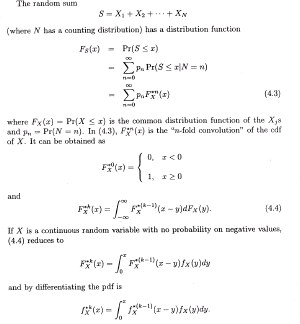
\includegraphics[width=0.6\textwidth]{ldachar}
\end{figure}


%% The random sum

%% \begin{equation}
%%   S = X_1 + X_2 + \cdots + X_N
%% \end{equation}

%% (where $N$ has a counting distribution) has a distribution function

%% \begin{equation}
%%   \begin{aligned}
%% F_s(x) &= P_x(S \leq x) \\
%%       &= \sum_{n=0}^{\infty}p_nP_x(S \leq x | N = n) \\
%%       &= \sum_{n=0}^{\infty}p_nF_X^n\{x\}
%%       \end{aligned}
%% \end{equation}

%% where $F_X(x) = P_x\{X \teq x\}$ is the common distribution function of the $X_j$ and $p_n = Px\{N = n\}$. In (d.3), $F_x^n\{x\}$ is the n-fold convolution of the cdf of $X$. It can be obtained as

%% smth

%% and

%% F_X^{\lambda}(X) = \int_{-\infty}^{\infty}

\subsection{Simulation method}

The goal is to determine the \emph{empirical} distribution function based on a sequence of (pseudo) random numbers $s_1, \ldots s_n$. Clearly, as the number of values increases, a more accurate estimate can logically be achieved. The risk horizon is usually taken as one year for operational risks. In the program, \emph{1000 simulations} are performed. We take the empirical values of their estimates (e.g. sample means, standard deviations, quantiles, etc.) as the characteristics of the distribution we are looking for. Confidence intervals of the estimates are not included in the calculation.


%------------------------------------------------

\section{Implementation of MC simulations}


\subsection{Excel program „MILDA\_E – Malý Ima LDA kalkulátor (Excel)“}

List and functionality of worksheets:
\begin{compactitem}

\item \textbf{Výběr}: shows list BL/ET (matrix k8x7 for banks), after
  the user makes a selection, it moves to the sheet:
\item \textbf{Vstupy\_a\_Výstupy}: for the selected BL/ET combination, the inputs and the calculation of the output values are introduced
\emph{vstupy} - the number of loss phenomena $N$, the probability of loss phenomena $p$, the coefficient $\lambda$ of the Poisson distribution, the average loss and variance of the loss distribution, the confidence limit $\alpha$,
\emph{výstupy} IMA - capital contribution of type \textbf{a} (with knowledge of loss severity variance) and \textbf{b} (without knowledge of loss severity variance), expected total loss
  
Sheet contains an LDA softkey that moves the calculation to the next \textbf{simulation phase}.
\item \textbf{Poisson\_distr.}: contains calculations based on the Poisson distribution
The last two sheets are complemented by the Normal distribution of the loss weights.
\item \textbf{Simulace}: This is the sheet in which the computations of the composite distribution are performed. The empirical frequency and loss magnitude distributions are generated (using pseudo-random numbers) and displayed. The computation problem focuses on generating random upper bounds for the summed sn values. An algorithm has been prepared that converts the random numbers generated from the Poisson distribution of occurrences into the computation of random upper bounds for the summation cells. These summation values (in aggregate) produce an empirical distribution of aggregate losses. In addition, the mean, standard deviation, 0.999 percentile and, by inference, the op. item, capital contribution to operational risk coverage are calculated.
\textbf{Simulace (2)}: is a sheet in which the calculated values of the characteristics of the composite distribution are displayed

\end{compactitem}

\subsection{Program characteristics}

The calculation uses Excel's statistical and lookup functions, including Visual Basic macros within Excel. The calculation is supported by a number of simulation libraries to generate pseudo-weighted numbers from prescribed distributions. It is not a limitation (due to the use of other analytic functions) to compute the Binomial distribution for large $N * p$ product, also Poisson $r$. for high $³ Lambda$. However, it is a limitation to use such values to compute simulations. For $\mu$, $\sigma$ the restriction of values is not required by the algorithm.

\subsection{Input/output sheets of the MILDA\_E application}

\begin{figure}[H]
  \caption{Matrix BL $\times$ ET}
  \centering
    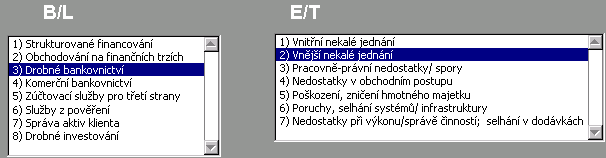
\includegraphics[width=0.75\textwidth]{matice}
\end{figure}


\begin{figure}[H]
  \caption{Risk capital summary table}
  \centering
    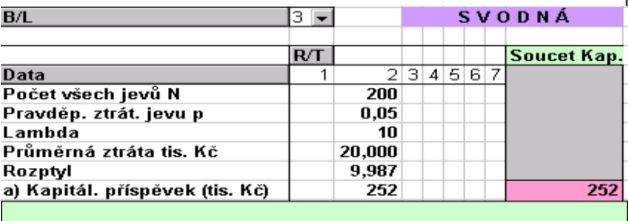
\includegraphics[width=0.75\textwidth]{tabulka}
\end{figure}

\begin{figure}[H]
    \caption{Input parameter of Poisson (active, red input) and lognormal distribution, to „LDA" calculation input}
  \centering
    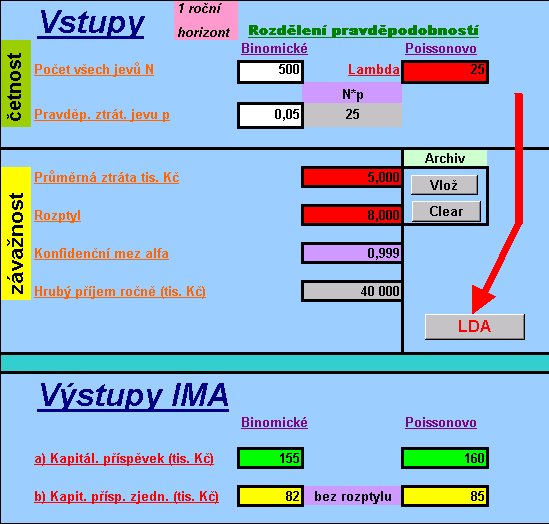
\includegraphics[width=0.75\textwidth]{vstup}

\end{figure}

\begin{figure}[H]
  \caption{„simuluj" calculation control button, simulation graph and risk characteristics (risk capital)}
  \centering
    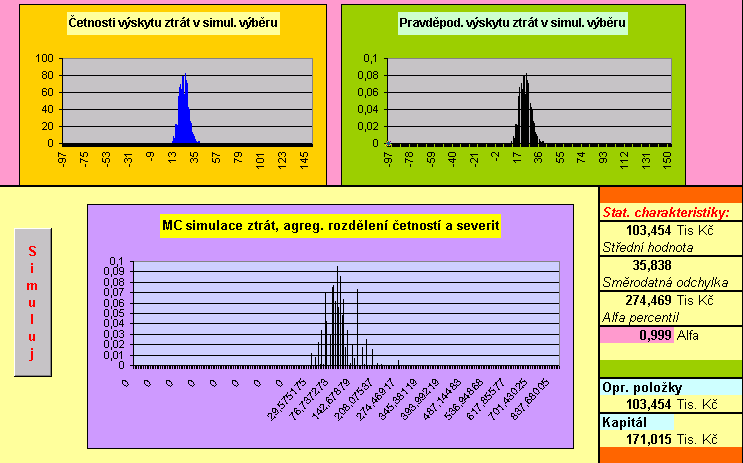
\includegraphics[width=0.75\textwidth]{simuluj}
\end{figure}


%----------------------------------------------------------------------------------------

%\end{multicols}

\end{document}
